
\documentclass[11pt]{article}
\usepackage[margin=1in]{geometry}
\usepackage{caption} %For captioning objects
\usepackage{subcaption} %sub-captioning pictures
\usepackage{graphicx} %to include graphics
\usepackage{hyperref} %for clickable references
\usepackage{listings} %to write code listings
\lstset{language=R, breaklines=true}  
\usepackage[mathcal]{euscript} %for curly S
\usepackage{mathtools}
\usepackage{float} %so figures can be placed "here"

%Defining commands for math symbols
\usepackage{amsmath} %to enable split equations
\usepackage{statmath} %for plim. Be careful, it has already \E and \V.
\usepackage{amssymb} %to enable mathbb
\newcommand{\R}{\mathtt{R}} %Software R
\renewcommand{\E}{\mathbb{E}} %expectation
\usepackage{bbm}
\newcommand{\1}{\mathbbm{1}}
\renewcommand{\V}{\mathbb{V}} %variance
\newcommand{\N}{\mathcal{N}} %normal distribution
\newcommand{\U}{\mathcal{U}} %normal distribution
\renewcommand{\P}{\mathbb{P}} %proba, renewcom since \P already exists
%Regression variables in vector form
\newcommand{\y}{\boldsymbol{y}} 
\newcommand{\x}{\boldsymbol{x}} 
\newcommand{\z}{\boldsymbol{z}} 
\newcommand{\yhat}{\boldsymbol{\hat{y}}} 
\renewcommand{\u}{\boldsymbol{u}} 
\newcommand{\uhat}{\boldsymbol{\hat{u}}}  
\newcommand{\Px}{\boldsymbol{P}}  
\newcommand{\Mx}{\boldsymbol{M}}  
\newcommand{\A}{\boldsymbol{A}}  
\newcommand{\X}{\boldsymbol{X}}  
\newcommand{\Z}{\boldsymbol{Z}}  
\newcommand{\e}{\boldsymbol{e}}  
\renewcommand{\r}{\tilde{r}}  
%\renewcommand{\r}{\boldsymbol{r}} 
\renewcommand{\i}{\boldsymbol{\imath}} 
\newcommand{\alphab}{\boldsymbol{\alpha}}  
\newcommand{\betab}{\boldsymbol{\beta}}  
%opening

\newcounter{daggerfootnote}
\newcommand*{\daggerfootnote}[1]{%
	\setcounter{daggerfootnote}{\value{footnote}}%
	\renewcommand*{\thefootnote}{\fnsymbol{footnote}}%
	\footnote[2]{#1}%
	\setcounter{footnote}{\value{daggerfootnote}}%
	\renewcommand*{\thefootnote}{\arabic{footnote}}%
}


\title{Problem Set 6 - ECON 880\\
	\small Spring 2022 - University of Kansas}
\author{Gunawan, Minh Cao}


\begin{document}

\maketitle	
\section*{Question 1}
We want to approximate $\int_0^1x^{\frac{1}{3}}dx$ using (A) Trapezoid rule, (B) Gauss-Chebyshev quadrature, and (C) Gauss-Legendre quadrature. We use $n\in\{3,5,11\}$ nodes with each approach. The true value of the integral is 0.75. The formula for each method is given below:
\begin{itemize}
\item The Trapezoid rule: Let $h=(b-a)/n$, $x_i=a+ih$, and $f_j\equiv f(x_j)$, then
$$\int_{a}^{b} f(x) d x\doteq\frac{h}{2}\left[f_{0}+2 f_{1}+\cdots+2 f_{n-1}+f_{n}\right]$$
\item The Gauss-Chebyshev quadrature:
$$
\int_{a}^{b} f(y) d y \doteq \frac{\pi(b-a)}{2 n} \sum_{i=1}^{n} f\left(\frac{\left(x_{i}+1\right)(b-a)}{2}+a\right)\left(1-x_{i}^{2}\right)^{1 / 2}
$$
where $x_i$'s are the Gauss-Chebyshev quadrature nodes over $[-1,1]$:
$$
x_{i}=\cos \left(\frac{2 i-1}{2 n} \pi\right), \quad i=1, \ldots, n .
$$
\item The Gauss-Legendre quadrature:
$$
\int_{a}^{b} f(x) d x \doteq \frac{b-a}{2} \sum_{i=1}^{n} \omega_{i} f\left(\frac{\left(x_{i}+1\right)(b-a)}{2}+a\right),
$$
where the $\omega_i$ and $x_i$ are the Gauss-Legendre quadrature weights and nodes over $[-1,1]$\daggerfootnote{See Kenneth L. Judd, 1998. "Numerical Methods in Economics," MIT Press Books, The MIT Press, p.260, Table 7.2}.
\end{itemize}
The relative error of the integral approximations is defined here as $|\hat{I}-I|/I$, where $\hat{I}$ and $I$ is the true approximated and the value of the integral, respectively. See Table \ref{tab:1} for results.

\begin{table}[H]
	\centering
\begin{tabular}{ |l||c|c|c|  }
 \hline
               & $n=3$ &$n=5$&$n=11$\\
 \hline
    Trapezoid      & 0.081359     &0.041771 &   0.01481\\
     Gauss-Chebyshev   &     0.036964    & 0.012382     &0.0024208\\
 Gauss-Legendre   &0.0051406   & 0.0015098 & 0.00020904\\
  \hline
\end{tabular}
	\caption{Relative errors of the integral approximations}
\label{tab:1}
\end{table}
Comment: We see that for the three approaches, the more we add the number of nodes, the lower the relative errors become. Out of the three methods, Gauss-Legendre quadrature performs best with the lowest relative errors, followed by Gauss-Chebyshev, and finally the Trapezoid rule.

\section*{Question 2}
We want to approximate $\int_{[0,1]^3}e^{x+2y +3z} dx dy dz$ using (A) pseudo-random numbers from Matlab’s rand(), (B) uniformly
spaced grid. For (A), we use the number of draws of the form $100n$ with $n = 1, 2,\ldots, 30$. For (B), we use $n$ equally spaced nodes along each dimension with $n^{1/3}=5,6,7,\ldots,14$. The true value of the integral is 34.920804.

The relative error of the integral approximations is defined here as $|\hat{I}-I|/I$, where $\hat{I}$ and $I$ is the true approximated and the value of the integral, respectively. See Figure \ref{fig:1} and \ref{fig:2} for relative errors resulting from method A and B, respectively.

Comment: On Figure \ref{fig:1}, we see that Method (A) exhibits no clear pattern of diminishing relative error towards zero, however it is bounded by roughly 0.075. On Figure \ref{fig:2}, it is clear that uniformly spaced grid method yields relative error that consistently decreases towards zero as $n$ increases. However, with the number of nodes less than 3000, the pseudo-random method performs better than the uniformly spaced grid since the relative error's lower bound of the uniformly spaced grid method is roughly 0.8, achieved at $n=14^3=2,744$ nodes. On the contrary, a relative error of 0.75 has been achieved using method (A) by choosing only $n=1,100$ nodes. From implementation point of view, it is easier to use Matlab's pseudo-random number generator, since we do not need, as in contrast to the other method, to divide all the three intervals into small grids and evaluate the function value at all of the grid points.  

\begin{figure}[h]
	\centering
		\includegraphics[width=5in]{fig2.eps}
	\caption{Relative Error for Method (A)}
	\label{fig:1}
\end{figure}
\begin{figure}[h]
	\centering
		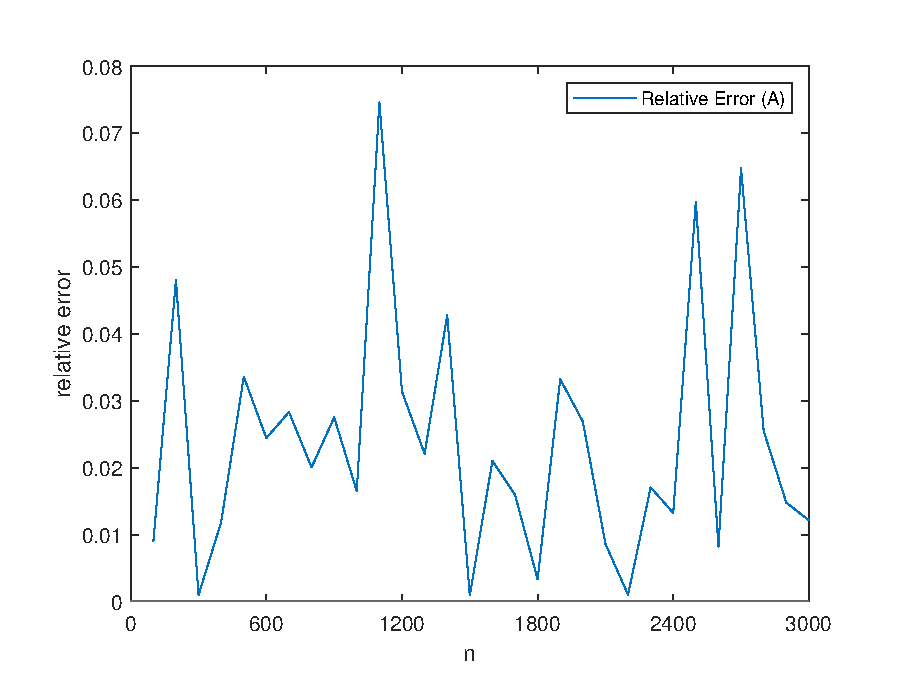
\includegraphics[width=5in]{fig1.eps}
	\caption{Relative Error for Method (B)}
	\label{fig:2}
\end{figure}

\end{document}

